% TestVDB — API compliance defect detector for VDBMSs (2026-07-11)

\documentclass[sigconf]{acmart}

% ACM conference metadata (placeholders — update for your target venue)
\setcopyright{acmlicensed}
\copyrightyear{2026}
\acmYear{2026}
\acmConference[Conference'26]{Proceedings of the ACM Conference}{June~2026}{Location}
\acmISBN{978-1-4503-XXXX-X/2026/06}
\acmDOI{10.1145/nnnnnnn.nnnnnnn}

\usepackage{booktabs}
\usepackage{graphicx}
\usepackage{amsmath}
\usepackage{listings}
\usepackage{xcolor}
\usepackage{enumitem}
\usepackage{tikz}
\usetikzlibrary{positioning, arrows.meta, calc}

\lstdefinestyle{curl}{
  basicstyle=\ttfamily\scriptsize,
  breaklines=true,
  keywordstyle=\color{blue},
  stringstyle=\color{teal},
  frame=single,
}

\begin{document}

\title{TestVDB: Detecting API Compliance Defects in Vector Database Systems via Contract-Truth Separation}

% Author anonymized for review
\author{Anonymous Author(s)}
\affiliation{%
  \institution{Submission \#XXX}
  \country{}
}

\ccsdesc[500]{Software and its engineering~--~Software testing and debugging}
\ccsdesc[300]{Information systems~--~Specialized database management systems}

\keywords{Vector database, API compliance defects, LLM-driven testing, test oracle, contract hallucination, multi-agent verification}

\begin{abstract}
Vector Database Management Systems (VDBMSs) underpin Large Language Model (LLM) applications, yet incorrect-behavior defects---43\% of VDBMS bugs---lack practical oracles, as current fuzzers detect only crashes. We target \emph{API compliance defects}: bugs where a VDBMS silently accepts inputs or behaviors that violate its documented contract. We present \textbf{TestVDB}, the first LLM-driven detector for them. TestVDB auto-derives a contract oracle from API documentation and applies \textbf{Contract-Truth Separation} (CTS), isolating LLM-generated assertions from a truth layer that falsifies them via maintainer-authority evidence; CTS is motivated by \emph{contract hallucination propagation}---when one LLM family both generates a contract and judges compliance, hallucinated constraints are self-confirmed. TestVDB produced issues across five VDBMSs, adjudicated on Milvus and Qdrant; maintainers acknowledged 36. On a controlled retrospective, the dev-reviewer's source anchor lifts false-positive suppression from 31\% to 81\% while retaining 96.7\% of true positives.
\end{abstract}

\maketitle

%=========================================================================
\section{Introduction}\label{sec:intro}

VDBMSs such as Milvus, Qdrant, Weaviate, Chroma, and MeiliSearch now underpin retrieval-augmented generation, recommendation, and multimodal search. As they enter production at scale, their reliability directly affects downstream decisions. A study of 1{,}671 bug-fix pull requests across 15 VDBMSs~\cite{bugstudy25} finds that more than half of all defects are functional failures; a complementary testing roadmap~\cite{roadmap25} reports that \emph{incorrect-behavior} bugs (43.0\%) substantially outnumber crash/hang bugs (23.1\%).

Despite this distribution, current VDBMS testing skews toward the minority. VDBFuzz~\cite{vdbfuzz26}, the first dedicated VDBMS fuzzer, uses crash as its oracle and detects only crash/hang bugs, leaving the majority without a practical oracle. The roadmap~\cite{roadmap25} flags this as the central open challenge: incorrect behavior ``poses significant challenges for test oracles,'' and approximate vector search renders traditional differential testing unsuitable. Its Future Work asks both for ``an oracle for evaluating the correctness of vector search results'' and for methods that let LLMs ``stay updated with the latest syntax and functionalities.''

We target a tractable slice of this gap: \emph{API compliance defects}---bugs where the VDBMS silently accepts an input or produces a behavior that violates its documented contract (e.g., accepting \texttt{nprobe=0}, silently normalizing \texttt{shardsNum=-1}, or returning success where the docs prescribe rejection). These bugs do not crash, but they corrupt query semantics, lower recall, and expand the attack surface. Crucially, they admit an oracle where general result-correctness does not: the API contract itself.

\paragraph{Why an LLM, and why that is not enough.}
Compliance defects produce no observable failure signal. Prior oracles are not useless---differential, metamorphic, and property-based testing address the mathematical-invariant and crash subsets of VDBMS behavior, and we reuse that subset (\S\ref{sec:eval-rq3})---but none reaches the compliance residual, because an accept/reject decision against a natural-language contract cannot be compiled into a deterministic assertion (Table~\ref{tab:exclusion}). The only oracle whose judgment spans this residual is an LLM, and REST-API doc-derived assertion oracles keep a deterministic checker and therefore stay out of this regime. Entering the regime is what makes one LLM family both \emph{generate} the contract and \emph{judge} compliance---and both can hallucinate.

\begin{table}[t]
\caption{Oracle candidates by the defect class they reach, and why the API-compliance residual forces an LLM-as-checker. Rows 1--4 use a deterministic checker; row 5 (REST doc/spec-derived assertion oracles) also keeps a deterministic checker and so never enters the LLM-as-checker regime; only row 6 is forced into it.}
\label{tab:exclusion}
\small
\begin{tabular}{@{}p{0.26\columnwidth}p{0.34\columnwidth}p{0.30\columnwidth}@{}}
\toprule
Candidate oracle & Reaches (defect class) & Why it misses the compliance residual \\
\midrule
Crash (VDBFuzz~\cite{vdbfuzz26}) & crash/hang & compliance defects do not crash \\
Differential testing & math invariants across vendors (our model-free subclass, \S\ref{sec:eval-rq3}) & cross-vendor accept/reject diverges by design; no compliance reference~\cite{roadmap25} \\
Metamorphic relations~\cite{metmap24} & result correctness (top-$k$ monotonicity, recall vs.\ $ef$) & an MR is an output relation; compliance is an input accept/reject decision---no transform preserves it \\
Property-based testing~\cite{claessen00,schemathesis,quickrest20} & math properties + schema conformance & needs a machine-checkable property and an OpenAPI schema; VDB endpoints serve neither \\
REST doc/spec-derived oracles (AGORA+, SATORI, MASTOR) & status/field/invariant assertions from OpenAPI or source & require OpenAPI or treat code as truth; checked deterministically, so they do not enter the LLM-as-checker regime \\
\textbf{LLM-as-checker (TestVDB)} & \textbf{accept/reject vs.\ documented contract} & \textbf{compliance semantics are not compilable to a deterministic assertion, forcing an LLM checker---the reliability problem this introduces is the subject of the next paragraph} \\
\bottomrule
\end{tabular}
\end{table}

\paragraph{Core reversal: the oracle itself may be wrong.}
The naive design---an LLM extracts a contract from docs, then the same family of models judges compliance against it---is brittle because of \emph{contract hallucination propagation}. We observed a concrete instance: the formalizer ``extracted'' a complexity requirement from \texttt{constant.go} that is in fact a guard against a historical performance regression, not a behavioral constraint; the judge then confirmed violations against it. Across our submissions, 12 of the 48 non-rejected adjudicated issues (acknowledged or by-design, i.e., 52 adjudicated minus 4 rejected; 25\%) were marked by-design: the LLM-derived contract was stricter than the maintainers' true intent (demanding rejection of idempotent duplicate creates, eventual-consistency staleness, or lenient defaults). When the same model family generates the contract and judges compliance, hallucinated constraints are self-confirmed.

\paragraph{Approach: Contract-Truth Separation.}
When no mechanical oracle is available, the only usable truth source is \emph{maintainer authority}---source code, prior PRs, by-design intent, issue history. It is scarce, so it must be proxied by an agent. We separate the \emph{assertion layer} (LLM-generated contracts and judgments) from a \emph{truth layer} and use the latter to falsify the former. The truth layer is a dev-reviewer agent that applies counter-evidence along three anchors: clean reproduction, source-grounded verification (the direct counter to hallucination), and threat-model cross-check. This mirrors how a maintainer adjudicates an incoming bug report.

\paragraph{Results.}
TestVDB produced 111 candidate issues across five VDBMSs, with adjudicated validation on Milvus and Qdrant and breadth probes on three further systems; maintainers acknowledged 36 (28 fixed, 8 accepted-open). On a controlled retrospective over all 52 maintainer-adjudicated candidates (same population), the dev-reviewer's source anchor lifts false-positive suppression from 31\% to 81\% while retaining 96.7\% of true positives ($n{=}30$); aggregated over the adjudicated pool (concentrated on Milvus and Qdrant; Weaviate, MeiliSearch, and Chroma are breadth probes), maintainer-adjudicated precision is 69.2\% (36/52, Wilson 95\% CI $[55.7\%, 80.1\%]$); under pending-resolution sensitivity the worst-case bound widens to $[43.9\%, 80.5\%]$ (Section~\ref{sec:eval-rq3}). We report the boundary honestly: 75\% of yield is boundary/validation compliance; crash bugs are excluded by design (complementary to VDBFuzz); soft result-correctness (ANN recall, ranking) remains open.

\paragraph{Positioning.}
We respond to VDBFuzz's generation-side Future Work (LLM-generated diverse API interactions and staying current with evolving APIs). Our judgment side provides a contract oracle that extends detection beyond crash into the API-compliance subset of incorrect behavior. We do \emph{not} claim to solve VDBFuzz's oracle-for-correctness direction (result correctness of vector search), which remains open~\cite{roadmap25}.

\paragraph{Contributions.}
\begin{enumerate}[leftmargin=*,itemsep=2pt]
\item The \textbf{first LLM-driven realization and empirical study of VDBMS API-compliance defect detection}: TestVDB is the first end-to-end system for non-crash compliance defects on the agenda of~\cite{roadmap25}, producing 111 submissions across five VDBMSs---adjudicated on Milvus and Qdrant (36 maintainer-acknowledged, 28 fixed)---with a reproducible open-source dataset; three further VDBMSs serve as breadth probes on the attack surface.
\item \textbf{Contract-Truth Separation (CTS)}: a design principle that isolates LLM-generated assertions from a maintainer-authority truth layer and falsifies them via source-grounded verification, motivated by \emph{contract hallucination propagation}---when one LLM family both generates a contract and judges compliance, hallucinated constraints are self-confirmed (25\% of adjudicated submissions were by-design). The dev-reviewer's source anchor lifts FP suppression from $31\%$ to $81\%$ at $96.7\%$ TP retention; the threat-model anchor is ablated as a noisy complement (\S\ref{sec:eval-tm}).
\item A \textbf{model-free invariant oracle subclass}---\texttt{COSINE} distance $>1.0$ for identical vectors, incomplete index results, payload-filter violations---that violates hard mathematical bounds, needs no LLM judgment, and reproduces across Milvus and Qdrant; it is adoptable independent of TestVDB's LLM pipeline.
\end{enumerate}

%=========================================================================
\section{Background and Problem Formulation}\label{sec:bg}

\subsection{VDBMS Architecture}
A VDBMS stores, indexes, and queries dense vector embeddings across a storage engine, a vector index (HNSW, IVF, etc.), a query processor (search, filtered/predicated search, multi-vector search), and client SDKs exposing REST and gRPC APIs~\cite{roadmap25}. Our targets live at the API surface and the query-processing logic behind it.

\subsection{Bug Taxonomy and Our Scope}
We adopt the symptom-level taxonomy of~\cite{roadmap25} as our primary frame (Crash/Hang 23.1\%, Incorrect Behavior 43.0\%, Others 15.0\%, Build 9.7\%, Performance 9.3\%) and corroborate it with the larger empirical study~\cite{bugstudy25} (5 symptom categories, 31 fault patterns) used as a fault-pattern vocabulary. Our compliance-dimension axis projects onto the symptom axis as in Table~\ref{tab:scope}: we operate inside Incorrect Behavior, specialize in its boundary/validation subset, and exclude Crash (by design), Performance, and Build.

\begin{table}[t]
\caption{TestVDB scope projected onto the roadmap symptom taxonomy~\cite{roadmap25}.}
\label{tab:scope}
\small
\begin{tabular}{@{}p{0.42\columnwidth}p{0.48\columnwidth}@{}}
\toprule
Symptom class (share) & TestVDB coverage \\
\midrule
Crash/Hang (23.1\%) & Out of scope (L1 gate filters; 1 incidental in yield) \\
Incorrect Behavior (43.0\%) & \textbf{In scope}: boundary/validation (75\% of yield) + diagnostic + state/logic subsets \\
Performance (9.3\%) & Out of scope \\
Build (9.7\%) & Out of scope \\
Others (15.0\%) & Out of scope \\
\bottomrule
\end{tabular}
\end{table}

\subsection{API Compliance Defects}
An \emph{API compliance defect} is a behavior where, for an input governed by a documented or implementable contract, the VDBMS (i) accepts an input the contract prescribes to reject (\emph{illegal success}), (ii) rejects or mishandles an input the contract prescribes to accept, or (iii) returns a response whose status, payload, or side effects violate the contract (\emph{poor diagnostics / state violation}). The contract is not assumed perfect; Section~\ref{sec:hallucination} confronts contract unreliability directly.

\subsection{The Oracle Problem}
Compliance defects produce no crash and no exception, and---unlike SQL---there are no widely-agreed reference semantics for VDBMS APIs across vendors. Differential testing is effective on mathematical invariants---our model-free subclass (\S\ref{sec:eval-rq3}) is precisely differential across vendors---but cannot adjudicate compliance, where accept/reject behavior diverges across vendors by design and no reference exists~\cite{roadmap25}. Metamorphic relations~\cite{metmap24} address result correctness but cannot reach accept/reject decisions: a metamorphic relation is an output relation, not an input-acceptance transform. The contract itself is the only candidate oracle for the residual---but it must be obtained and trusted, which is the core problem we address.

%=========================================================================
\section{Approach}\label{sec:approach}

\subsection{Overview}
TestVDB is a five-stage pipeline (Figure~\ref{fig:overview}): (1) contract extraction from API documentation via an LLM knowledge-extractor; (2) attack generation by specialized agents guided by a threat-model prior; (3) a four-judge debate producing Stage-2 candidates; (4) a dev-reviewer that applies Contract-Truth Separation as counter-evidence; (5) a two-layer novelty gate. A threat-model artifact is reused across stages as an experience prior.

\paragraph{Implementation.} All agents are LLM-driven and served by GLM-5.2; four heavy-reasoning agents (orchestrator, dev-reviewer, threat-modeler, bug-shape-extractor) run on the high-budget configuration and the remaining sixteen on the low-budget configuration---both the same GLM-5.2 backbone, differing in context window and max output tokens rather than model families. Four independent judges (evidence, novelty, severity, documentation) score each Stage-2 candidate; the orchestrator aggregates their verdicts and forwards survivors to the dev-reviewer, which suppresses a candidate if any of its three anchors (clean reproduction, source-grounding, threat-model) yields counter-evidence. An end-to-end trace (contract hallucination $\to$ source-grounded reclassification) appears in \S\ref{sec:hallucination}.

\paragraph{Reproducibility and cost.} Target VDBMS versions are pinned per system (Milvus 2.6.19 for the single-LLM and single-layer ablations; the full version matrix is in the artifact). The pipeline is orchestrated by the Claude Code runtime, which dispatches each agent to the GLM-5.2 backbone under its default sampling configuration (no explicit temperature override), and each of the 20 agents is defined by a task-structured role prompt (full prompts in the artifact). A full pipeline run per target invokes the 20 agents over $O(10\text{--}50)$ generated attack candidates; wall-clock is dominated by the dev-reviewer's source-grounding step (repository clone and source retrieval) and live Docker re-probes rather than raw LLM latency. The 111-submission study plus three ablation batches (52-candidate retrospective, 15-probe single-layer A1, 15-probe single-LLM B9) constitutes the full LLM-call budget; in aggregate this is on the order of $10^4$ LLM calls ($\sim$$10^7$ tokens); per target, a full pipeline (contract extraction through dev-reviewer) costs on the order of $10^3$ calls ($\sim$$2{\times}10^6$ tokens) and completes in a few hours (on the order of \$10 per target at current LLM API pricing, comparable to a few hours of manual boundary testing). For this cost, TestVDB's marginal value over a hand-written boundary fuzzer is threefold: non-boundary yield (state/logic, diagnostic, result-correctness probes), source-grounded FP-suppression across all categories, and spec-gap detection where the doc is silent (\S\ref{sec:eval-rq3}). This threefold value is anchored by \emph{5 unique TPs} (3 diagnostic-quality, 2 state/logic) that the full pipeline reaches but our 19-probe boundary fuzzer and the model-free invariant oracle do not: the 2 state/logic cases are unreachable by \emph{any} stateless single-response oracle, while the 3 diagnostic cases are a lower bound relative to this probe instance, not a fuzzer-class upper bound (Table~\ref{tab:incremental}). Precise per-token and wall-clock accounting is part of the anonymized artifact at \url{https://anonymous.4open.science/r/testvdb-anon-D644/}, to be made public on acceptance.

\begin{figure}[t]
\centering
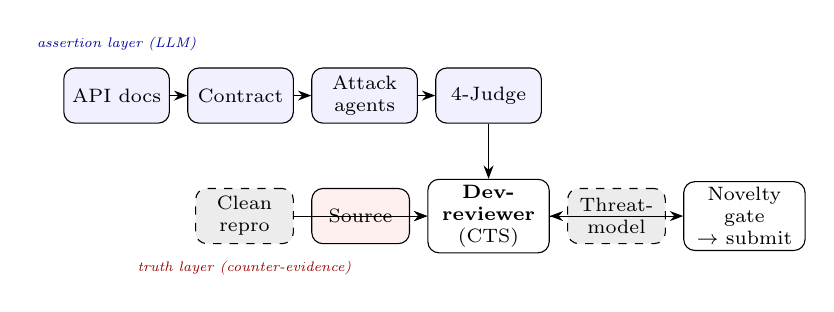
\begin{tikzpicture}[
  node distance=2.2mm and 2.2mm,
  font=\scriptsize,
  assert/.style={draw, rounded corners, fill=blue!6, align=center, inner sep=2pt, text width=12mm, minimum height=7mm},
  truth/.style={draw, rounded corners, fill=red!6, align=center, inner sep=2pt, text width=11mm, minimum height=7mm},
  truthunval/.style={draw, rounded corners, dashed, fill=gray!15, align=center, inner sep=2pt, text width=11mm, minimum height=7mm},
  gate/.style={draw, rounded corners, align=center, inner sep=2pt, text width=14mm, minimum height=7mm},
  arr/.style={-Stealth, thin}
]
\node[assert] (docs) {API docs};
\node[assert, right=of docs] (contract) {Contract};
\node[assert, right=of contract] (attack) {Attack\\agents};
\node[assert, right=of attack] (judge) {4-Judge};
\node[gate, below=7mm of judge] (devrev) {\textbf{Dev-reviewer}\\\scriptsize(CTS)};
\node[truth, left=of devrev] (src) {Source};
\node[truthunval, left=of src] (repro) {Clean\\repro};
\node[truthunval, right=of devrev] (tm) {Threat-\\model};
\node[gate, right=of tm] (out) {Novelty gate\\$\to$ submit};
\draw[arr] (docs)--(contract);
\draw[arr] (contract)--(attack);
\draw[arr] (attack)--(judge);
\draw[arr] (judge)--(devrev);
\draw[arr] (repro)--(devrev);
\draw[arr] (src)--(devrev);
\draw[arr] (tm)--(devrev);
\draw[arr] (devrev)--(out);
\node[font=\tiny\itshape, color=blue!60!black] at ($(docs.north)+(0,3mm)$) {assertion layer (LLM)};
\node[font=\tiny\itshape, color=red!60!black] at ($(repro.south)+(0,-3mm)$) {truth layer (counter-evidence)};
\end{tikzpicture}
\caption{TestVDB pipeline. The assertion layer (LLM contract + 4-judge) is falsified by the dev-reviewer's three counter-evidence anchors (truth layer): the \emph{source} anchor (solid) is the primary, validated anchor; the \emph{threat-model} anchor (dashed, optional) is ablated in \S\ref{sec:eval-tm} as a noisy offline complement on $n{=}12$ Milvus FPs (unstable; catches boundary-default residuals but over-fires on state/concurrency); the \emph{reproduction} anchor (gray, dashed) remains design-level and not yet evaluated. CTS = Contract-Truth Separation.}
\label{fig:overview}
\end{figure}

\subsection{Contract Extraction and the Threat-Model Prior}\label{sec:tm}
A knowledge-extractor agent crawls official API documentation and emits structured contracts (parameter domains, enum values, documented limits, status-code semantics) that seed both attack agents and judges. A threat-model artifact encodes recurring by-design intents (idempotency, eventual consistency, lenient defaults) and known blind spots. It is \emph{designed} to be injected at generation, judgment, and dedup; however, in our runs the blindspot indicators were never populated and its effect could not be isolated (Section~\ref{sec:eval-tm}), so we treat it as an unvalidated optional prior rather than a working component of the evaluated system.

\subsection{Attack Generation and the Four-Judge Debate}
Three attack agents target the compliance dimensions: a \emph{boundary} agent (illegal-success at parameter, enum, and limit edges---the dominant yield), a \emph{semantic} agent (diagnostic-quality violations), and a \emph{state} agent (state/logic inconsistencies). Candidates enter a four-judge debate (evidence/severity/novelty/doc axes) drawing on multi-agent verification ideas~\cite{du2023improving}. The Stage-2 output of this debate feeds the dev-reviewer.

\subsection{Contract-Truth Separation and the Dev-Reviewer}\label{sec:cts}
Single-layer LLM judgment is unreliable because the same model family generates the contract and judges compliance. CTS breaks this self-confirmation by introducing an independent truth layer. The dev-reviewer agent proxies maintainer authority and falsifies each Stage-2 candidate along three anchors:
\begin{itemize}[leftmargin=*,itemsep=2pt]
\item \textbf{Clean reproduction.} Build a minimal reproducer against a live VDBMS of the pinned target version; reject candidates whose ``defect'' is a tooling artifact (we withdrew early candidates that misread a missing \texttt{rowCount} field as ``returns $-1$'').
\item \textbf{Source-grounded verification.} Locate the implementation behind the API and check whether the observed behavior is intended---the direct counter to contract hallucination (Section~\ref{sec:hallucination}).
\item \textbf{Threat-model cross-check.} Match against known by-design intents before flagging a violation.
\end{itemize}
This mirrors maintainer adjudication: most of our false positives stem from contracts stricter than true intent, and source grounding is what exposes them. Of the three anchors, we validate source-grounding as the primary anchor in the controlled retrospective (\S\ref{sec:eval-rq3}); the threat-model anchor is ablated as a noisy complement (\S\ref{sec:eval-tm}); the reproduction anchor remains design-level future work.

\paragraph{Dev-reviewer prompt.} The dev-reviewer is a double-blind, suspicion-first falsifier. Its access is restricted to raw HTTP request/response logs (the sole source of truth), the candidate list (defect metadata only---other judges' votes and rationales are hidden), the structured contract, and a developer-cognition model; it is explicitly forbidden from reading the attack scripts' assertion logic, which is exactly what it must independently re-derive. For each Critical/High candidate it executes a six-step SOP: (1) clean-room reproduction from a rebuilt minimal request (via Bash, not imagined); (2) assumption audit---a ``violation'' resting on a response field the request never requested is void; (3) contract grounding with mandatory source re-verification (formalizer confidence fields are not trusted); (4) independent-channel falsification (e.g., primary-key \texttt{GET} or \texttt{scroll} to recover the ground-truth set); (5) mundane-explanation exclusion (race, eventual consistency, parameter typo); (6) structured verdict---\texttt{CONFIRMED} only if all steps pass and step-1 reproduction succeeds. Four hard constraints enforce double-blind access, Bash execution in steps 1 and 4, contract citation, and a suspicion-first default. Full prompts are in the artifact.

\subsection{Novelty Gate}
A two-layer gate prevents re-reporting: L1 checks local history and the threat-model blind-spot set; L2 queries the target repository's issues and PRs. Candidates surviving both are submitted.

%=========================================================================
\section{Contract Hallucination Propagation}\label{sec:hallucination}
We highlight a phenomenon that, to our knowledge, has not been characterized in LLM-driven testing. When an LLM generates the contract \emph{and} judges compliance, hallucinated constraints are not caught by the judge---they are produced by the same generation--judgment family and thus inherit mutual confirmation. We observed two forms.

\textbf{(1) Fabricated provenance.} The formalizer produced a ``complexity requirement'' attributed to \texttt{constant.go}; source grounding showed the constant guards a past performance regression, not a behavioral constraint. The Stage-2 judge nonetheless confirmed violations against it.

\textbf{(2) Over-strict intent.} 12 of the 48 substantively adjudicated submissions (25\%) were marked by-design: the contract demanded rejection of behaviors maintainers intended to allow---idempotent duplicate creates returning success, eventual-consistency staleness, lenient naming defaults, and silent enum/empty substitutions.

Formally, let $C_{\mathrm{LLM}}$ be the LLM-derived contract and $C_{\mathrm{true}}$ the maintainer intent. Single-layer judgment assumes $C_{\mathrm{LLM}} = C_{\mathrm{true}}$; when $C_{\mathrm{LLM}} \supset C_{\mathrm{true}}$ (stricter), genuine by-design behaviors are flagged as violations, and the judge---sharing the generator's bias---does not dissent. The dev-reviewer's source-grounded anchor is the mitigation: it reintroduces an external truth signal ($C_{\mathrm{true}}$ proxied by source and history). We present this as a qualitative characterization; a quantitative study of hallucination frequency is future work, and the 12 by-design cases are direct observations rather than a measured rate over all inputs.

%=========================================================================
\section{Evaluation}\label{sec:eval}

We address three primary research questions (RQ1--RQ3) and report one exploratory negative result (RQ4, Section~\ref{sec:eval-tm}).

\subsection{RQ1: Detection Capability}
We ran TestVDB against five VDBMSs, pinning exact target versions (Table~\ref{tab:yield}). Yield concentrates on Milvus (51 submissions) and Qdrant (26); MeiliSearch (3) and Chroma (1) contribute near-zero adjudicated signal, so our cross-system generalization is claimed primarily for Milvus and Qdrant, with Weaviate, MeiliSearch, and Chroma as breadth rather than statistical evidence.

\begin{table}[t]
\caption{Issues submitted and maintainer outcomes (5 VDBMSs). 52 of the 111 submissions have been adjudicated (36 acknowledged $=$ 28 fixed $+$ 8 accepted, 12 by-design, 4 rejected). Of the remaining 59, 30 are \emph{pending} (open, awaiting triage) and drive the sensitivity interval in Section~\ref{sec:eval-rq3}; 29 are \emph{excluded} (closed-no-label or duplicate, unresolvable) and lie outside that interval.}
\label{tab:yield}
\small
\begin{tabular}{lrrrrrrr}
\toprule
VDBMS & Sub. & Fix. & Acc. & ByD. & Rej. & Pend. & Excl. \\
\midrule
Milvus      & 51 & 14 & 8 & 12 & 0 & 0  & 17 \\
Qdrant      & 26 & 11 & 0 & 0  & 3 & 8  & 4 \\
Weaviate    & 30 & 3  & 0 & 0  & 1 & 21 & 5 \\
MeiliSearch & 3  & 0  & 0 & 0  & 0 & 0  & 3 \\
Chroma      & 1  & 0  & 0 & 0  & 0 & 1  & 0 \\
\midrule
\textbf{Total} & \textbf{111} & \textbf{28} & \textbf{8} & \textbf{12} & \textbf{4} & \textbf{30} & \textbf{29} \\
\bottomrule
\end{tabular}
\end{table}

\paragraph{Defect-type distribution.} Of the 36 acknowledged true positives, 27 (75\%) are boundary/validation, 3 (8\%) diagnostic-quality, 2 (6\%) state/logic, 1 (3\%) crash, and 3 (8\%) result-correctness. The result-correctness cases are instructive: they include \texttt{COSINE} distance returning $>1.0$ for identical vectors (a hard mathematical-invariant violation, reproduced on both Milvus and Qdrant), incomplete index results (2 of 25 matching points returned), and a payload filter returning points with a missing field. These are detectable because they violate expressible invariants; soft result-correctness (ANN recall/ranking error) remains open. \emph{Incremental yield by oracle class:} of the 36 TPs, 27 boundary/validation are in principle reachable by a spec-driven fuzzer (our 19-probe instance found 5 genuine violations); 3 result-correctness by the model-free invariant oracle; 1 crash by a crash oracle (VDBFuzz's domain). The remaining \textbf{5 TPs---3 diagnostic-quality and 2 state/logic---are reachable only by the full LLM pipeline}, as they need semantic judgment over undocumented behavior or multi-step state sequences; Table~\ref{tab:incremental} lists each by GitHub issue and verifies \emph{per-defect} why neither the 19-probe boundary fuzzer (stateless single-parameter values) nor the model-free invariant oracle (per-response math bounds) reaches it. We also ran the 19-probe fuzzer on milvus v2.6.19: none of its 19 probes triggers any of the three milvus TPs (the probe set has no load$\to$search sequence, no malformed-filter probe, and no delete endpoint), backing the milvus subset by execution rather than argument; the two non-milvus TPs are out of the fuzzer's scope by construction. The two claims differ in strength: the two state/logic cases are unreachable by \emph{any} stateless single-response oracle---they require multi-step state sequences or cross-parameter logic---whereas the three diagnostic-quality cases are unreachable by \emph{our} 19-probe instance in particular, and a larger or differently designed probe set could plausibly reach some. The ``5'' is therefore a lower bound relative to this instance, not a fuzzer-class upper bound. Beyond these 5 unique TPs, CTS FP-suppression lifts end-to-end precision from $45.6\%$ (the single-layer counterfactual of \S\ref{sec:eval-rq3}: one live, source-grounded adjudication cycle without CTS---distinct from the $25.5\%$ Single-LLM self-judgment rate) to $69.2\%$, a cross-category contribution neither the spec fuzzer nor the model-free oracle provides.

\begin{table}[t]
\caption{The 5 acknowledged TPs reachable only by the full LLM pipeline (3 diagnostic-quality, 2 state/logic). For each, neither our 19-probe boundary fuzzer instance (stateless single-parameter boundary values: nprobe/ef/limit=0, $-1$; dimension out-of-range; consistencyLevel/metricType enum substitution; required-field omission) nor the model-free invariant oracle (per-response math bounds: \texttt{COSINE}$\in[-1,1]$, index completeness, payload-field presence) reaches the trigger. Last column: we ran the 19-probe fuzzer on milvus v2.6.19---\emph{0/19} probes trigger each milvus TP (the probe set has no load$\to$search sequence, no malformed-filter probe, and no delete endpoint), and the fuzzer is milvus-only so the two non-milvus TPs are out of scope. State/logic cases are unreachable by any stateless oracle; diagnostic cases by this instance in particular (text).}
\label{tab:incremental}
\small
\begin{tabular}{@{}llp{0.33\columnwidth}p{0.14\columnwidth}@{}}
\toprule
TP & Class & Why both baselines miss it & 19-probe run \\
\midrule
milvus \#47636 & diag. & expr parser returns code=0 and leaks lexer errors; error-semantics, not a parameter boundary, no math bound & 0/19 \\
qdrant \#9039 & diag. & async upsert silent-discards a dim-mismatched vector; needs a follow-up GET, not a single-response bound & milvus-only \\
weaviate \#12041 & diag. & batch delete returns HTTP 500 not 422; status-code semantics, no math bound & milvus-only \\
milvus \#47635 & state & search returns code=0 right after \texttt{load()}; requires a load$\to$search state sequence & 0/19 \\
milvus \#50323 & state & delete accepts both \texttt{filter} and \texttt{ids} (documented mutually exclusive); a logic constraint & 0/19 \\
\bottomrule
\end{tabular}
\end{table}

\paragraph{Complementarity with VDBFuzz.} Our yield is almost entirely non-crash (35/36); VDBFuzz's crash oracle---its title frames the problem as ``Crash Bugs''~\cite{vdbfuzz26} and its source contains no compliance-checking logic---cannot detect non-crash defects, so at most 1/36 of our yield (the single crash case) could overlap with VDBFuzz's targets. Conversely, our L1 gate deliberately filters crash-prone inputs, so TestVDB does not target the crash bugs VDBFuzz finds. The complementarity follows from the oracle definitions; a head-to-head empirical comparison on identical targets is future work.

\subsection{RQ2: Case Studies}
We trace three end-to-end cases that span the TP/FP boundary and the dev-reviewer's role, then isolate a model-free oracle subclass.
\textbf{True positive, correctly surfaced (Milvus \#47729).} An invalid \texttt{nprobe}=0 was accepted by search. The attack agent derived the probe from the contract; the four-judge debate confirmed it; the dev-reviewer's source anchor raised no counter-evidence (no documented lower bound); the maintainer fixed it.
\textbf{True positive, correctly surfaced (Milvus \#49844).} An empty filter silently triggered a full scan; same path; maintainer accepted.
\textbf{False positive, correctly suppressed (Milvus \#50193).} \texttt{get\_stats} returned \texttt{rowCount}=0 immediately after insert. The four-judge confirmed it as a bug; the dev-reviewer's source anchor reclassified it as documented eventual consistency (async aggregation; 0 is a valid intermediate)---precisely the consistency-semantics FP class the source anchor targets---and the maintainer later closed it as by-design, confirming the reclassification.
\paragraph{Model-free invariant oracles.} The \texttt{COSINE} distance returned $>1.0$ for identical vectors, independently reproduced on both Milvus and Qdrant. Unlike the contract-driven cases above, this violates a \emph{mathematical invariant} (cosine similarity is bounded in $[-1,1]$) and needs no LLM judgment---an expressible, model-free oracle subclass worth distinguishing from contract oracles. The same class catches incomplete index results (2/25 matching points returned) and payload filters returning points with a missing field. This subclass is the paper's most defensible technical finding: it depends on no LLM judgment, reproduces across vendors, and violates a hard mathematical bound, so it is the least contingent on the agent-design choices the rest of the evaluation rests on.

\subsection{RQ3: Precision --- Controlled Retrospective and Aggregate}\label{sec:eval-rq3}

\subsubsection{Controlled Retrospective}
We re-triaged all 52 maintainer-adjudicated candidates (36 TP, 16 FP) under two blind conditions on the \emph{same} population: claim-only (4-judge layer) vs.\ source-grounded (dev-reviewer's source anchor), outcomes hidden via label-isolated agents. Source-grounding lifts FP suppression from 5/16 ($31\%$) to 13/16 ($81\%$, $2.6\times$)---Milvus $33\%{\to}75\%$, non-Milvus $0\%{\to}100\%$---while retaining 29/30 TPs ($96.7\%$; 6 TPs were unreachable via API rate limits). This same-population comparison is our primary evidence for the dev-reviewer's contribution.

\subsubsection{Aggregate Precision}
Across five VDBMSs, 52/111 submissions are adjudicated (36 acknowledged, 12 by-design, 4 rejected). Counting by-design and rejected as maintainer-judged FPs,
\[
\mathrm{precision}_{\mathrm{adj}} = \frac{\mathrm{acknowledged}}{\mathrm{acknowledged}+\mathrm{by\text{-}design}+\mathrm{rejected}} = \frac{36}{36+12+4} = 69.2\%.
\]
This is an end-to-end operating point (Wilson 95\% CI $[55.7\%, 80.1\%]$ on $n{=}52$), not the ``after'' arm of the retrospective above (different population and denominator).

\subsubsection{Sensitivity Analysis}
Of 59 unadjudicated submissions, 30 are pending and 29 are excluded (closed-no-label or duplicate). As a bound on the 29 excluded: if all were false positives, precision over the 81 non-pending drops to $36/81{=}44.4\%$; if all were true positives, it rises to $65/81{=}80.2\%$. For the 30 pending: all-valid gives $(36{+}30)/82=80.5\%$, all-invalid gives $36/82=43.9\%$. Over the adjudicated 52, the Wilson 95\% CI is $[55.7\%, 80.1\%]$; the wider $[43.9\%, 80.5\%]$ is therefore a worst-case bound over unadjudicated submissions, not a statistical CI on the headline estimate.

\subsubsection{Baseline Comparisons}
\textbf{Within-system (same 52 pool).} Claim-only lets 11/16 FPs through (judgment-layer precision $33/44=75\%$); source-grounded lets $3/16$ through ($29/32=91\%$).\footnote{The two conditions use slightly different TP denominators (claim-only scored all 36; source-grounding scored 30 reachable via the GitHub API, 6 rate-limited), within the same 52-candidate pool.}

\textbf{Single-layer counterfactual (A1).} Removing the FP-suppression chain and re-running generation + 4-judge debate on milvus v2.6.19 confirmed 3 candidates (2 TP: \#47729 invalid \texttt{nprobe}=0, \#49844 empty-filter full scan; 1 FP: \#50193 eventual-consistency).

\textbf{Live FP audit (27 killed candidates).} To bound the arm's FP inflow without LLM-proxy judgment, we re-probed all 27 dev-reviewer-killed candidates live on a fresh v2.6.19 container and source-grounded each via milvus constants (\texttt{DefaultConsistencyLevel=ClBounded}, \texttt{DefaultShardNumber=0}); all 27 reproduce as true FPs (\emph{27/27 live, over-kill $0/27$}).

\textbf{Derived single-layer precision.} Combining the 27 suppressed with the $36/52$ baseline gives single-layer precision $36/(36{+}16{+}27)=45.6\%$ vs.\ TestVDB's $69.2\%$. This $45.6\%$ rests on live + source grounding (not LLM-proxy); we report it as a directional lift at zero recall cost, treating the same-population $31\%\to 81\%$ as the cleaner head-to-head.

\textbf{Single-LLM.} A single LLM end-to-end (no multi-agent debate, no CTS) produced 51 candidates, 13 LLM-judged TP ($25.5\%$, Wilson $[15.5\%, 38.9\%]$); a source-grounded self-judgment filter drops it to $11.8\%$ ($6/51$, $[5.5\%, 23.4\%]$) after by-design reclassification. Note the construction differs from the single-layer counterfactual above: that arm keeps the full multi-agent generation and 4-judge debate and removes only the FP-suppression chain ($45.6\%$), whereas this arm removes the multi-agent debate entirely ($25.5\%$). Both remain far below $69.2\%$, so multi-agent debate plus CTS contributes beyond source anchoring alone.

\textbf{Schema-aware boundary fuzzer.} A hand-written boundary fuzzer (19 probes, no LLM) surfaced 7 API-accepted candidates; source-grounded post-filter classifies 5 as genuine violations ($71\%$) and 2 as by-design defaults. This concedes that on the boundary/validation subset ($75\%$ of yield) a spec-driven fuzzer is effective. TestVDB's marginal value lies where the fuzzer cannot reach: (a) non-boundary probes (state/logic, diagnostic, result-correctness: $8/36$ TPs); (b) CTS FP-suppression (the fuzzer has no source-grounded layer); (c) spec-gap bugs where the doc is silent. A Schemathesis head-to-head is blocked (Milvus serves no standards-compliant OpenAPI; \texttt{/swagger}, \texttt{/openapi.json} all 404).

Rows across arms use different ground truths (LLM self-judgment / API-acceptance / blind re-triage / maintainer), so they are \emph{not} directly comparable across tiers; Table~\ref{tab:baselines} and Figure~\ref{fig:precision} make the asymmetry explicit rather than drawing cross-tier conclusions.

\subsubsection{Anchor Attribution}
On the 16 FPs, the \emph{source} anchor drives the full lift (claim-only $5/16=31\%$; adding source $13/16=81\%$); the 3 residuals are silent-absent cases (no validation code to cite). The \emph{threat-model} anchor (\S\ref{sec:eval-tm}): source-alone $9/12$, threat-alone $6/12$ (unstable), union $11/12$, TP $4/4$ throughout---threat catches 2 source residuals (boundary-default) but over-fires on state/concurrency (\textsc{bs-}03/06). The \emph{reproduction} anchor needs a live container and is not exercised here. Source is primary; threat-model is a noisy complement; reproduction is future work.



\begin{table}[t]
\caption{Precision/ground-truth comparison across arms, grouped by truth tier (weak proxy $\to$ maintainer gold). Rows are \emph{not} directly comparable across tiers (different ground truths); the retrospective and maintainer tiers share the same 52-candidate pool. CI is Wilson 95\%. The last row's worst-case pending-resolution bound $[43.9\%, 80.5\%]$ (Section~\ref{sec:eval-rq3}) is drawn separately in Figure~\ref{fig:precision} and is not a statistical CI on the adjudicated subset. $^{\dagger}$The schema-fuzzer 37\% is a probe$\to$accept rate (7 of 19 probes surfaced an API-accepted candidate), not a candidate precision; source-grounded post-filter classifies 5 of those 7 as genuine violations ($71\%$, live-confirmed on a fresh v2.6.19 container).}
\label{tab:baselines}
\small
\begin{tabular}{@{}llccl@{}}
\toprule
Arm & Precision & $n$ & Ground truth (tier) & 95\% CI \\
\midrule
\multicolumn{5}{@{}l}{\emph{LLM-judged (weak proxy)}} \\
Single-LLM & 25.5\% & 51 & LLM self-judgment & [15.5\%, 38.9\%] \\
Single-LLM + source filter & 11.8\% & 51 & LLM + source & [5.5\%, 23.4\%] \\
\midrule
\multicolumn{5}{@{}l}{\emph{API-acceptance (weak proxy)}} \\
Schema fuzzer (no LLM) & 37\%$^{\dagger}$ & 19 & API-acceptance & --- \\
\midrule
\multicolumn{5}{@{}l}{\emph{Retrospective (same 52-candidate pool, blind judge)}} \\
Single-layer 4-judge & 75\% & 44 & claim-only re-triage & --- \\
TestVDB source-grounded & 91\% & 32 & source re-triage & --- \\
\midrule
\multicolumn{5}{@{}l}{\emph{Maintainer adjudication (gold)}} \\
TestVDB (end-to-end) & 69.2\% & 52 & maintainer triage & [55.7\%, 80.1\%] \\
\bottomrule
\end{tabular}
\end{table}

\begin{figure}[t]
\centering
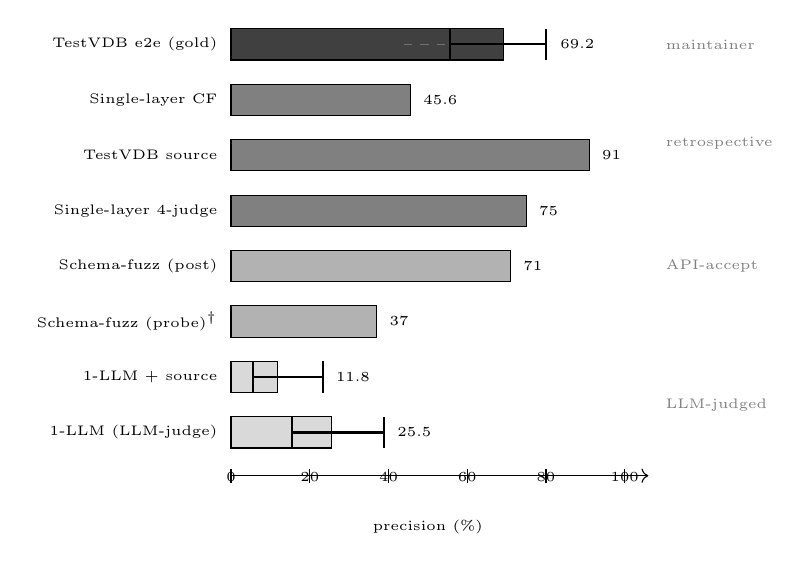
\begin{tikzpicture}[font=\tiny, yscale=0.88]
% x-axis (precision 0-100 -> 0-5cm)
\draw[->] (0,-0.3) -- (5.3,-0.3);
\foreach \p in {0,20,40,60,80,100} {
  \pgfmathsetmacro\xx{\p*0.05}
  \draw (\xx,-0.4) -- (\xx,-0.2) node[below=-2pt,font=\tiny]{\p};
}
\node[font=\tiny,below=10pt] at (2.5,-0.4) {precision (\%)};
% TestVDB end-to-end (maintainer gold) 69.2 Wilson [55.7, 80.1] solid; worst-case bound [43.9, 80.5] dashed
\draw[fill=black!75] (0,5.7) rectangle (3.46,6.15);
\draw[dashed,thin,black!55] (2.195,5.925) -- (4.025,5.925);
\draw[thick] (2.785,5.925) -- (4.005,5.925);
\draw[thick] (2.785,5.7) -- (2.785,6.15);
\draw[thick] (4.005,5.7) -- (4.005,6.15);
\node[anchor=east,font=\tiny] at (-0.05,5.925) {TestVDB e2e (gold)};
\node[anchor=west,font=\tiny] at (4.06,5.925) {69.2};
% Single-layer counterfactual (retrospective, directional) 45.6
\draw[fill=black!50] (0,4.9) rectangle (2.28,5.35);
\node[anchor=east,font=\tiny] at (-0.05,5.125) {Single-layer CF};
\node[anchor=west,font=\tiny] at (2.32,5.125) {45.6};
% TestVDB source-grounded (retrospective) 91
\draw[fill=black!50] (0,4.1) rectangle (4.55,4.55);
\node[anchor=east,font=\tiny] at (-0.05,4.325) {TestVDB source};
\node[anchor=west,font=\tiny] at (4.59,4.325) {91};
% Single-layer 4-judge (retrospective) 75
\draw[fill=black!50] (0,3.3) rectangle (3.75,3.75);
\node[anchor=east,font=\tiny] at (-0.05,3.525) {Single-layer 4-judge};
\node[anchor=west,font=\tiny] at (3.79,3.525) {75};
% Schema-fuzzer post-filter 71
\draw[fill=black!30] (0,2.5) rectangle (3.55,2.95);
\node[anchor=east,font=\tiny] at (-0.05,2.725) {Schema-fuzz (post)};
\node[anchor=west,font=\tiny] at (3.59,2.725) {71};
% Schema-fuzzer probe->accept 37 (dagger, not candidate precision)
\draw[fill=black!30] (0,1.7) rectangle (1.85,2.15);
\node[anchor=east,font=\tiny] at (-0.05,1.925) {Schema-fuzz (probe)$^\dagger$};
\node[anchor=west,font=\tiny] at (1.89,1.925) {37};
% Single-LLM + source 11.8 [5.5, 23.4]
\draw[fill=black!15] (0,0.9) rectangle (0.59,1.35);
\draw[thick] (0.275,1.125) -- (1.17,1.125);
\draw[thick] (0.275,0.9) -- (0.275,1.35);
\draw[thick] (1.17,0.9) -- (1.17,1.35);
\node[anchor=east,font=\tiny] at (-0.05,1.125) {1-LLM + source};
\node[anchor=west,font=\tiny] at (1.21,1.125) {11.8};
% Single-LLM (LLM-judged) 25.5 [15.5, 38.9]
\draw[fill=black!15] (0,0.1) rectangle (1.275,0.55);
\draw[thick] (0.775,0.325) -- (1.945,0.325);
\draw[thick] (0.775,0.1) -- (0.775,0.55);
\draw[thick] (1.945,0.1) -- (1.945,0.55);
\node[anchor=east,font=\tiny] at (-0.05,0.325) {1-LLM (LLM-judge)};
\node[anchor=west,font=\tiny] at (1.99,0.325) {25.5};
% tier grouping labels
\node[font=\tiny,gray,anchor=west] at (5.4,5.925) {maintainer};
\node[font=\tiny,gray,anchor=west] at (5.4,4.5) {retrospective};
\node[font=\tiny,gray,anchor=west] at (5.4,2.725) {API-accept};
\node[font=\tiny,gray,anchor=west] at (5.4,0.725) {LLM-judged};
\end{tikzpicture}
\caption{Precision by ground-truth tier (darker = stronger). Whiskers = Wilson 95\% CI; for TestVDB e2e the \emph{dashed} whisker is the pending-resolution worst-case bound $[43.9\%, 80.5\%]$ (\S\ref{sec:eval-rq3}), wider than its Wilson CI. $^\dagger$ = probe$\to$accept rate, not candidate precision. \emph{Bars in different tiers use different ground truths and are not directly comparable; compare only within a tier.} Details in Table~\ref{tab:baselines}.}
\label{fig:precision}
\end{figure}

\subsection{RQ4: Threat-Model Anchor --- Wired and Ablated}\label{sec:eval-tm}
An earlier double-blind ablation on Milvus v2.6.17 (control with threat-model cognition vs.\ experiment without; $n{=}5$ TP, 7 FP) returned an exploratory negative (TP recall 20\%/60\%; blindspot indicators never reached the dev-reviewer's consumption path; the agent was unstable across runs). On inspection, the negative was confounded by a wiring gap: the threat-modeler populated \texttt{threat\_model.json} with 6 cognitive blindspots and 10 by-design behaviors, but the dev-reviewer consumed \texttt{developer\_cognition.json}'s \texttt{blindspot\_indicators} field, which was empty. We re-ran the ablation with the wiring fixed (a v2 dev-reviewer prompt that reads \texttt{threat\_model.json} directly), on the 12 Milvus FPs of the retrospective plus 4 Milvus TPs as a recall control, under three conditions: \emph{source-alone} (network on, threat-model blanked), \emph{threat-alone} (network off, threat-model populated), and \emph{both} (union of the two independent verdicts). Source-alone suppresses 9/12 FPs ($75\%$); threat-alone suppresses 6/12 ($50\%$) and is unstable across runs (one boundary FP flipped between runs); their union (a candidate is suppressed if \emph{either} anchor independently flags it---an OR of two blind verdicts, not a joint dispatch requiring both to agree) suppresses 11/12 ($92\%$); all three conditions retain 4/4 TPs. The threat anchor catches 2 of source's 3 residuals (boundary-default cases where no validation code exists to cite) but misses 5 state/concurrency FPs that source catches---its blindspot mechanism (\textsc{bs-}03 concurrency, \textsc{bs-}06 state-consistency) over-fires there, pushing genuine by-design FPs toward CONFIRMED. The threat anchor is thus neither an offline substitute for source nor dead weight, but a \emph{noisy complement} whose value is the union. We do not claim the three-anchor design as a clean validated contribution on the strength of $n{=}12$; we report it as a diagnosed result that explains why source-grounding remains the primary anchor and bounds the threat anchor's standalone effect honestly.

\subsection{Threats to Validity}
\begin{itemize}[leftmargin=*,itemsep=2pt]
\item \textbf{Internal.} Maintainer acknowledgment is a weak ground truth; triage may reflect report clarity rather than defect validity.
\item \textbf{Selection.} The 111 submissions were filtered from a larger candidate pool by the novelty gate; the candidate-to-submission ratio is not instrumented, leaving submission-selection bias roughly bounded.
\item \textbf{External.} The same-population ablation (RQ3) is Milvus-plus-Qdrant only; Weaviate submissions are largely undiagnosed (21 of 30 remain pending/open, reflecting maintainer triage latency rather than substantive invalidation---none are rejected).
\item \textbf{Construct.} Defect-type classification is title-based, pending per-defect confirmation.
\item \textbf{LLM variance.} Re-adjudicating the 46 source-grounded candidates five times with independent agents yields $99.1\%$ pairwise agreement and $45/46$ unanimous verdicts; residual variance sits upstream in version-pinned source extraction.
\item \textbf{Contamination.} GLM-5.2 may have seen pre-2024 Milvus source in training. A memorization canary (bare model, no docs) recalls general bug-class knowledge (e.g., ``cosine $\in [-1,1]$'') but \emph{0/9} held-out issues at issue-specificity, so the 9-bug cohort is not memorization-confounded; we flag the cosine$>$1 invariant as the one overlap with general mathematical knowledge rather than count it as independent evidence. A contract counterfactual (DeepSeek on the same doc passages) reproduces over-strict constraints in $2/9$ of an expanded $N{=}10$ set---partly task-intrinsic on default-as-value cases but predominantly GLM-specific, which CTS targets directly.
\item \textbf{Recall scope.} The $96.7\%$ figure is judgment-layer TP retention, not end-to-end discovery recall. To measure recall directly, we ran a held-out rediscovery study on 9 pre-2024 compliance bugs (qdrant/weaviate/milvus, GLM-5.2 training-data-external): for each, we started the bug-present version in Docker, derived the contract from that version's API docs, and probed whether the attack reproduces the violation (simplified recall: contract derivation + targeted probe, not the full 20-agent pipeline). TestVDB \textbf{rediscovered $4/9$} ($44\%$, Wilson 95\% CI $[18.9\%, 73.3\%]$ on $n{=}9$---wide, but its lower bound clears a trivial zero-discovery baseline; $4/7{=}57\%$ of the testable subset, $2$ blocked by milvus/pymilvus SDK incompatibility): qdrant silent-accept of wrong vector size (v1.5.0), qdrant incorrect validation of \texttt{max\_indexing\_threads} (v1.2.0), weaviate silent-accept of trailing JSON junk (v1.19), and weaviate silent-ignore of unrecognized query params (v1.19). These $4$ are independent held-out bugs (canary: 0/9 recalled at issue-specificity), so this is genuine discovery recall, not memorization. Two bugs were already fixed in the tested version; two deeper limits bound the rest: \emph{spec-completeness} (qdrant dimension-mismatch invisible to spec-derived contract) and \emph{version-pinning} (milvus cosine$>$1.0 fixed before release).
\item \textbf{Excluded set.} 17 of the 29 excluded submissions are Milvus; closed-no-label may reflect maintainer non-engagement rather than invalidity, so excluding them could hide an FP tail (bounded in \S\ref{sec:eval-rq3}: worst case $36/81{=}44.4\%$).
\item \textbf{Single-layer counterfactual.} The $45.6\%$ figure combines the maintainer-adjudicated $36/52$ baseline with 27 live-re-probed FPs; triage might reclassify a few of the 27, and the arm is bounded to one feedback cycle.
\end{itemize}

%=========================================================================
\section{Related Work}\label{sec:rw}
\paragraph{VDBMS testing.} VDBFuzz~\cite{vdbfuzz26} is the first dedicated VDBMS fuzzer (crash-oracle-based) and is complementary to this work. The roadmap~\cite{roadmap25} and the empirical bug study~\cite{bugstudy25} define the agenda and taxonomy we build upon. MeTMaP~\cite{metmap24} applies metamorphic testing to false vector matching in LLM-augmented generation. BUZZBEE~\cite{buzzbee24} fuzzes general DBMSs.
\paragraph{REST API and schema testing.} RESTler~\cite{restler19} infers producer--consumer dependencies among REST request types for stateful fuzzing; EvoMaster~\cite{evomaster21} evolves REST API test sequences. Schemathesis~\cite{schemathesis} applies property-based testing directly to OpenAPI/GraphQL schemas to surface contract violations, and QuickREST~\cite{quickrest20} derives property-based tests from OpenAPI serving as both generator and oracle; both require a standards-compliant specification---which VDBMS REST endpoints do not serve (we probe \texttt{/swagger}, \texttt{/openapi.json}, and related paths in \S\ref{sec:eval-rq3}, all returning 404), so schema-driven fuzzers cannot be applied off-the-shelf. More recent REST fuzzers---foREST~\cite{lin2023forest}, MINER~\cite{lyu2023miner}, and DynER~\cite{chen2024dyner}---advance sequence/parameter-value generation but remain OpenAPI-driven with 5XX/crash oracles; none targets semantic compliance against the documented contract. These tools target schema-conformance and crash at the API boundary; we extend the boundary to \emph{semantic} compliance (does the response honor the documented contract?) and to VDBMS-specific invariants.
\paragraph{Database correctness oracles.} NoREC~\cite{norec20} tests SQL via a non-optimizing reference engine; TLP~\cite{tlp20} partitions queries three ways; DQE~\cite{dqe20} pivots query execution; DDLCheck~\cite{ddlcheck25} targets DDL correctness. These assume reference SQL semantics absent in VDBMS APIs; our contract oracle replaces reference SQL with documentation-derived invariants.
\paragraph{LLM-based testing and verification.} LLMs increasingly drive test generation and software-engineering tasks~\cite{hou23llmse}, and multi-agent LLM systems are surveyed comprehensively by He et al.~\cite{he2025lma}; we use multi-agent debate~\cite{du2023improving} for generation and judgment. A key difference from prior LLM-as-judge patterns is that we identify a self-confirmation failure mode when one model family both generates the contract and judges compliance---the contract-hallucination phenomenon (\S\ref{sec:hallucination}). The contract-hallucination failure mode we identify is a spec-extraction instance of LLM hallucination more broadly~\cite{ji23hall}, mitigated in general by self-consistency~\cite{wang22sc}---we instantiate the mitigation as source-grounded falsification rather than prompt-level consensus. Concurrent LLM-driven REST testing (LlamaRestTest~\cite{kim2025llamaresttest}) fine-tunes a small LLM for input generation and dependency detection; our delta is orthogonal---CTS targets contract hallucination via maintainer-authority falsification, not input quality.
\paragraph{Test oracles and contracts.} The oracle problem is a long-standing concern~\cite{barr15}; our contract oracle is an instance of the \emph{specified} class and the cosine-bounded / completeness subclass is an instance of the \emph{derivable} class. Property-based testing~\cite{claessen00} and Design by Contract~\cite{meyer92dbc} are precursors of specification-driven checking; static API-misuse detection~\cite{amann19} targets client-side misuse, whereas we target server-side non-compliance. General fuzzing is surveyed in~\cite{manes21}.

%=========================================================================
\section{Conclusion and Future Work}\label{sec:conc}
We presented TestVDB, the first LLM-driven system for detecting API compliance defects in VDBMSs, built on Contract-Truth Separation. On a controlled retrospective over 52 candidates, the dev-reviewer's source anchor lifts false-positive suppression from 31\% to 81\% while retaining 96.7\% of true positives; aggregated maintainer-adjudicated precision is 69.2\% (within $[43.9\%, 80.5\%]$). \emph{Scope:} boundary/validation compliance, complementary to crash-focused fuzzing; result-correctness oracles (ANN recall) remain open. Contract hallucination propagation generalizes beyond VDBMSs: any system where one LLM family both extracts a spec and checks compliance is susceptible---REST API contract testing, configuration validation, and policy-as-code compliance wherever documentation is the only available oracle. CTS-style source-grounded falsification is the natural mitigation in each. All CTS results use a single model family (GLM-5.2); cross-model validation of contract-hallucination propagation and CTS effectiveness is the primary open direction. Future work: stronger dev-reviewer backbones, an empirical VDBFuzz comparison, cross-library ablation beyond Milvus and Qdrant, and a larger discovery-recall cohort beyond the 9 held-out bugs measured here ($4/9$ rediscovered).

%=========================================================================
\bibliographystyle{ACM-Reference-Format}
\bibliography{references}

\end{document}
